\documentclass[12pt]{article}
\usepackage{braket}
\usepackage{feynmp-auto}
\usepackage{amsmath}
\usepackage{amssymb}
\usepackage{graphicx}
\usepackage{dsfont}
\usepackage{commath}
\setlength\parindent{0pt}
\linespread{1.2}
\usepackage[a4paper, total={6.6in, 9in}]{geometry}
\title{Intro}
\author{Jarrick Nys}

\begin{document}
\maketitle
\section{Inleiding}

\begin{figure}[h!]
\centering
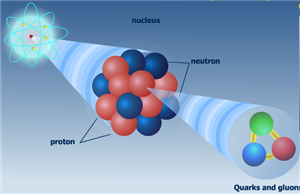
\includegraphics[scale=1]{Atom-Nucleus-Quark}
\end{figure}
Het atoom,  tot begin 19de eeuw bekend als de kleinste bouwsteen van het universum, werd later ontwaard als zijnde een kern met rondom een wolk van elektronen. De kern van een atoom is een zelf-gebonden systeem van nucleonen, waarij we een onderscheid kunnen maken tussen neutronen en protonen.  Het doel van deze thesis is kennis te verwerven over eigenschappen van dit systeem en in het bijzonder over de de impuls die de nucleonen bezitten. We bestuderen Impulsdistributies van nulceonen in atomaire kernen. Deze beschrijven hoe de impuls van een nucleon in de kern is verdeeld. Ze kunnen onder meer als input gebruikt worden bij simulaties van scattering experimenten aan nucleonen in een kern. Bij deze experimenten is het nodig om zo goed mogelijk de spectraalfunctie $P(\vec{k},\ E)$ te kennen van de te beschieten kern. De Spectraalfunctie $P(\vec{k},\ E)$ geeft de probabiliteit om een nucleon met impuls $\vec{k}$ te verwijderen waarbij de kern achterblijft met een excitatie-energie $E$. De \'{e}\'{e}ndeeltjes impulsdistributie $n_1(\vec{k})$ kan gerelateerd worden aan de spectraalfunctie via
\begin{equation}
n^{[1]}(\vec{k}) = \int dE \  P_1(\vec{k},E)
\end{equation} 
Een voorbeeld van dergelijk experiment is het Long-Baseline Neutrino Experiment (LBNE) waar ze gebruik maken van vloeibare-argon detectoren. Een optimale detectie vereist een goede kennis van he het neutrino-argon scatteringproces \cite{anderson2012first}. We bestuderen hier in het bijzonder $^{40}$Ar omdat \cite{ankowski2014} meldt dat er geen theoretische studies zijn van de impulsdistributies voor $^{40}$Ar.
We benaderen de nucleus met een gemiddeld-veld model. Nucleonen bewegen onafhankelijk van elkaar in een sferische harmonische oscillator portentiaal. Correlaties worden dus bij definitie verwaarloosd. De gemiddelde kinetische energie van de neutronen en protonen wordt bepaald aan de hand van de \'{e}\'{e}ndeeltjes momentumdistributie. De tweedeeltjes momentumdistributie wordt bestudeerd in functie van het relatieve momentum, massacentrum momentum en de hoek tussen deze.


\bibliographystyle{plain}
\bibliography{argoneutrino,ankowski}
\end{document}

